\documentclass[12pt]{report}
\usepackage{caption}
\usepackage{graphicx}
\usepackage{hyperref}
\hypersetup{%
    pdfborder = {0 0 0}
}
\hypersetup{
    colorlinks,
    citecolor=blue,
    filecolor=blue,
    linkcolor=blue,
    urlcolor=blue
}
\renewcommand{\familydefault}{\sfdefault}
\renewcommand{\captionfont}{\small}

\author{Bernd Porr}
\title{Realtime embedded coding under Linux}

\begin{document}

\maketitle

\tableofcontents

\chapter{Writing C++ device driver classes}

\begin{figure}[!hbt]
\begin{center}
\mbox{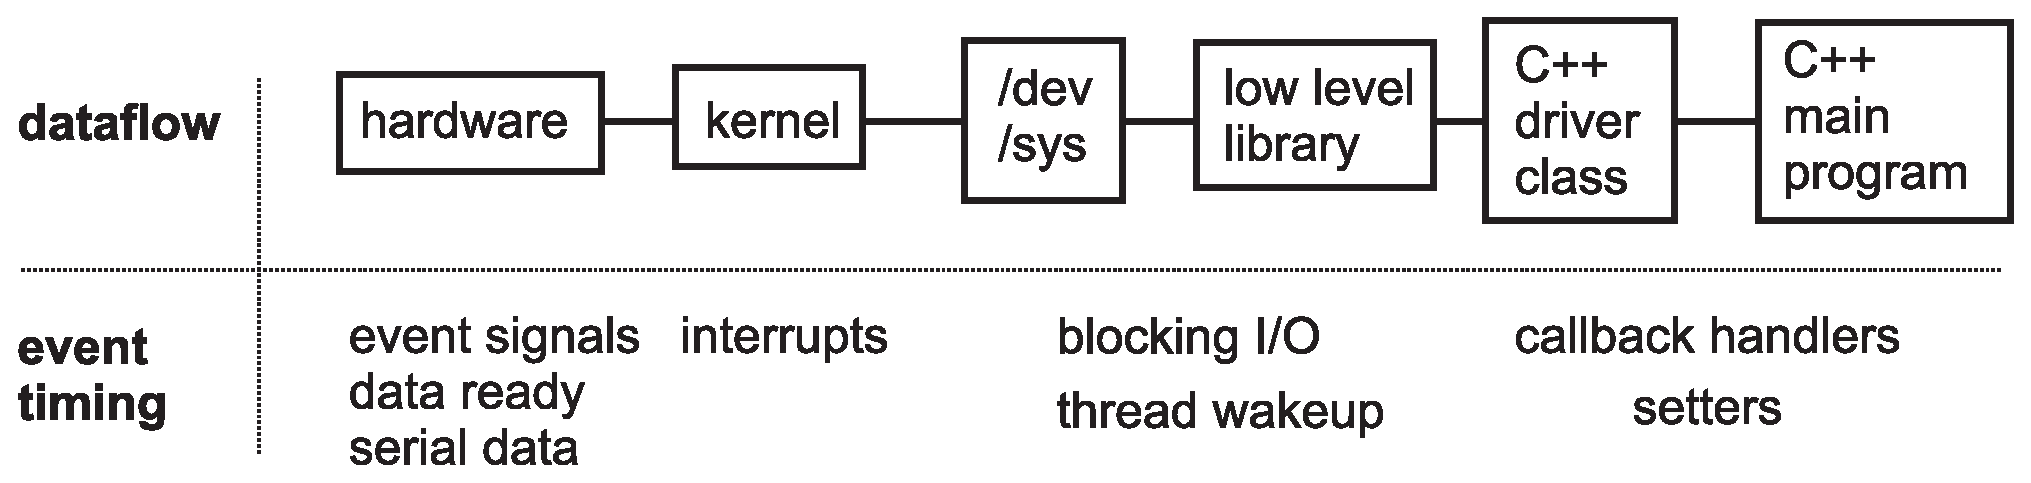
\includegraphics[width=\textwidth]{signals-timings}}
\end{center}
\caption{Dataflow and timing in low level realtime coding
\label{timing}}
\end{figure}

\section{Introduction}
Fig.~\ref{timing} shows the basic dataflow and how event timing is
established. While it's obvious that data needs to flow from/to the
hardware it's even more important to guarantee its timing in realtime
applications. On the hardware-side the timing is guaranteed by event
signals, data-ready signals and also by the timing of a serial
interface. The Linux kernel translates this timing info into blocking
I/O on pseudo filesystems such as /dev or /sys which means that a read
operation blocks till data has arrived or an event has happened. Some
low level libraries such as pigpio translate them back into C
callbacks.  Your task is to hide this complexity and these quite
different approaches in C++ classes which communicate via callbacks
and setters with the client classes.

\begin{figure}[!hbt]
\begin{center}
\mbox{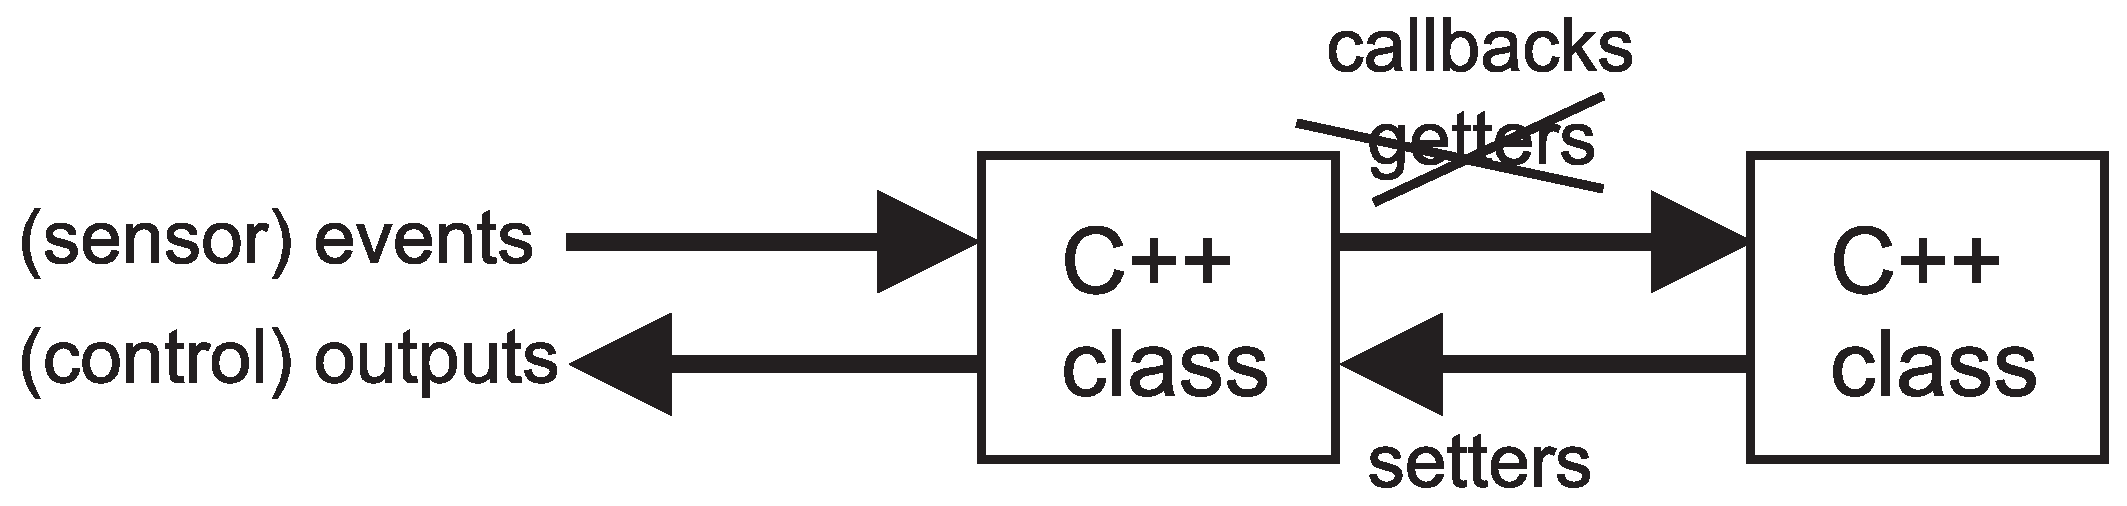
\includegraphics[width=\textwidth]{gettersetters}}
\end{center}
\caption{A realtime system with two C++ classes. Communication
  between classes is achieved with callbacks (not getters) for incoming events
  and setters to send out control events. The control output itself
  receives its timing from the events so that the loop is traversed
  as quickly as possible.
\label{gettersetters}}
\end{figure}
Fig.~\ref{gettersetters} shows the overall communication between C++
classes in a realtime system. This communication is done via callbacks
(\textsl{not} getters) and setters where an event from a sensor
traverses according to its realtime requirements through the classes via
callbacks and then back to the control output via setters. For example
a collision sensor at a robot triggers a GPIO pin, which then triggers a
callback to issue an avoidance action which in turn then sets the
motors in reverse.

This chapter focuses on writing your own C++ device driver class
hiding away the complexity (and messy) low level C APIs and/or raw
device access to /dev and /sys.


\section{General recommendations how to write your C++ classes for devices}
As said above the main purpose of object oriented coding here is to
hide away the complexity of low level driver access and offer the
client a simple and safe way of connecting to the sensor. In
particular:
\begin{enumerate}
\item Setters and callbacks hand over \textsl{physical units}
  (temperature, acceleration, \ldots) and not raw integer values which
  have no meaning.
\item The sensor is configured by specifying physical units (time,
  voltage, temperature) and not sensor registers. Default config parameters
  should be specified that the class can be used straight away with
  default parameters.
\item The class handles the realtime processing by offering callback
  interfaces (i.e. based on classes with virtual and abstract methods)
  to transmit data from the sensor and setters to transmit data to the device.
\item A build system is essential. It's strongly recommended to use ``cmake''
  (autoconf only for older existing projects).
\item The class is re-usable outwith of your specific project and has
  its own ``cmake'' project in a subdirectory and is a
  library.
\item It has doc-strings for all public functions and constants,
  has documentation generated by doxygen.
\item It has simple demo programs demonstrating how to use the class
  by a client.
\end{enumerate}

Keep S.O.L.I.D.
\url{https://www.digitalocean.com/community/conceptual_articles/s-o-l-i-d-the-first-five-principles-of-object-oriented-design}
in mind when writing your C++ device classes:
\begin{enumerate}
\item \textsl{Single responsibility}: If you have a temperature
sensor and an accelerometer then write two classes, one for the
temperature sensor and one of the accelerometer. In terms of
\item \textsl{Open-Closed principle} Your class is open to extension but
  closed to modification. For example an ADC class
  has a callback which returns voltage to the client. However,
  you'll be connecting for example a temperature sensor to
  it so you'd like to be able to extend the class by for example
  overloading the callback methods so that you add the conversion
  from volt to degrees but not hacking the existing ADC class.
\item \textsl{Liskov substitution principle} Any derived class from
  your device driver class can be used in place of the base class if
  the base class is all that's required, because the extra
  functionality in the derived class shouldn't break the basic
  required functionality of the base class. For example, if you have a
  super duper DAC with lots of extra features, it shouldn't stop you
  using it when you only need a very simple one. This also means
  that sensible default values should be set so that the client
  won't need to understand the nerdy features of that super duper DAC.
\item \textsl{Interface Segregation Principle}:
  Keep functionality separate and rather divide it up in different
  classes. Imagine you have a universal IO class with SPI and I2C
  but your client really just needs SPI. Then the client is forced
  to deactivate I2C or in the worst case the class causes collateral
  damage without the client knowing why.
\item \textsl{Dependency inversion}: That is about obstructing the
  essential features of of a class of interfaces. For example ideally
  you want, for example, a base class for covering a range of simuliar
  ADC converters from the same manufacturer and not a base class being
  a driver for a particular chip. Instead you want all ADC chip driver
  classes to inherit from the abstract ADC driver.
\end{enumerate}

\section{Low level userspace device access}
The following sections provide pointers of how to write
the C++ driver classes for different hardware protocols.

\subsection{SPI}
\begin{table}[!ht]
  \begin{center}
  \caption{SPI modes\label{spimodes}}
  \begin{tabular}{l|l|l|l}
    SPI Mode & 	CPOL & 	CPHA & Idle state \\
    \hline
    0& 	0&	0& 	L \\
    1& 	0&	1& 	L \\
    2& 	1&	1& 	H \\
    3& 	1&	0& 	H \\
  \end{tabular}
  \end{center}
\end{table}
SPI is a protocol which usually transmits and receives at the same
time. Even that data might not be used it needs to be matched up. So
for example sending 8 byes and recieving 8 bytes at the same time.

Transfer to/from SPI is best managed by the low level access to /dev.
Open the SPI device with the standard open() function:
\begin{verbatim}
int fd = open( "/dev/spidev0.0", O_RDWR);
\end{verbatim}

Then set the SPI mode (see table.~\ref{spimodes}):
\begin{verbatim}
int ret = ioctl(fd, SPI_IOC_WR_MODE, &mode);
\end{verbatim}
which is explained, for example, here:
\url{https://www.analog.com/en/analog-dialogue/articles/introduction-to-spi-interface.html}.

Since SPI transmits and receives at the same time we need to
use ioctl to do the communication.
Populate this struct:
\begin{verbatim}
struct spi_ioc_transfer tr = {
  .tx_buf = (unsigned long)tx1,
  .rx_buf = (unsigned long)rx1,
  .len = ARRAY_SIZE(tx1),
  .delay_usecs = delay,
  .speed_hz = speed,
  .bits_per_word = 8,
};
\end{verbatim}
which points to two character buffers ``tx'' and ``rx'' with the
same length.

Reading and simultaneous writing is happening then via the ioctrl
function:
\begin{verbatim}
int ret = ioctl(fd, SPI_IOC_MESSAGE(1), &tr);
\end{verbatim}

Sometimes the SPI protocol of a chip is so odd that even the raw
I/O via /dev won't work and you need to write your own bit banging
interface, for example done here for the ADC on the alphabot:
\url{https://github.com/berndporr/alphabot/blob/main/alphabot.cpp#L58}.
This is obviously far from ideal as it might require ``usleep'' commands
so that acquisition needs to be run in a separate thread (the alphabot
uses a timer callback in a separate thread).

Overall the SPI protocol is often device dependent and calls
for experimentation to get it to work. Often the SPI clock is also
the ADC conversion clock which requires a longer lasting clock signal
by transmitting dummy bytes in addition to the payload.

As a general recommendation do not use SAR converters which use the
SPI data clock also as acquisition clock as they are often not compatible
with the standard SPI transfers via /dev. Use sensors or ADCs which
have their own clock signal.


\subsection{I2C}
The I2C bus has two signal lines (SDA \& SDL) which must be pulled up
by resistors. Every I2C device has an address on the bus. You can scan
a bus with ``i2cdetect'' (part of the i2c-tools package):
\begin{verbatim}
root@raspberrypi:/home/pi# i2cdetect -y 1
     0  1  2  3  4  5  6  7  8  9  a  b  c  d  e  f
00:                         -- -- -- -- -- -- -- -- 
10: -- -- -- -- -- -- -- -- -- -- -- -- -- -- 1e -- 
20: -- -- -- -- -- -- -- -- -- -- -- -- -- -- -- -- 
30: -- -- -- -- -- -- -- -- -- -- -- -- -- -- -- -- 
40: -- -- -- -- -- -- -- -- -- -- -- -- -- -- -- -- 
50: -- -- -- -- -- -- -- -- 58 -- -- -- -- -- -- -- 
60: -- -- -- -- -- -- -- -- -- -- -- 6b -- -- -- -- 
70: -- -- -- -- -- -- -- --                         
root@raspberrypi:/home/pi# 
\end{verbatim}
In this case there are 3 I2C devices on the I2C bus at addresses
1E, 58 and 6B and need to be specified when
accessing the I2C device.

\subsubsection{Raw /dev/i2c access}
I2C either transmits or receives but never at the same time so here we
can use the standard C read/write commands. However, we need to use ioctrl to tell
the kernel the I2C address:
\begin{verbatim}
char buf[2];
int file = open("/dev/i2c-2",O_RDWR);
int addr = 0x58;
ioctl(file, I2C_SLAVE, addr);
write(file,buf,1)
read(file,buf,2)
\end{verbatim}
where ``addr'' is the I2C address. Then use standard read()
or write() commands. Usually the 1st write() operation tells the chip
which register to read or write to. Then write/read its register.

\subsubsection{I2C access via pigpio}
Access via pigpio (\url{http://abyz.me.uk/rpi/pigpio/cif.html})
is preferred in contrast to direct
access of the raw /dev/i2c because many different devices
can be connected to the I2C bus and pigpio manages this.
Simply install the development package:
\begin{verbatim}
sudo apt-get install libpigpio-dev
\end{verbatim}
which triggers then the install of the other relevant packages.
For example writing a byte to a register in an I2C sensor can be done with a
few commands:
\begin{verbatim}
int fd = i2cOpen(i2c_bus, address, 0);
i2cWriteByteData(fd, subAddress, data);
i2cClose(fd);
\end{verbatim}
where i2c\_bus is the I2C bus number (usually 1 on the RPI)
and the address is the I2C address of the device on that bus.
The subAddress here is the register address in the device.

\subsection{Access GPIO pins}
\subsubsection{/sys filesystem}
The GPIO of the raspberry PI can easily be controlled via
the /sys filesystem. This is slow but good for
debugging as you can directly write a
``0'' or ``1'' string to it and print the result. The
pseudo files are here:
\begin{verbatim}
/sys/class/gpio
\end{verbatim}
which contains files which directly relate to individual pins.
To be able to access a pin we need to tell Linux to make
it visible:
\begin{verbatim}
/sys/class/gpio/export
\end{verbatim}
For example, writing a 5 (in text form) to this file would
create the subdirectory \texttt{/sys/class/gpio/gpio5} for GPIO pin 5.

Then reading from
\begin{verbatim}
/sys/class/gpio/gpio5/value
\end{verbatim}
would give you the status of GPIO pin 5 and writing
to it would change it.
A thin wrapper around the GPIO sys filesystem is here: \url{https://github.com/berndporr/gpio-sysfs}.

\paragraph{GPIO interrupt handling via /sys\label{gpioIRQ}}
The most important application for the /sys filesystem is to
do interrupt processing in userspace.
A thread can be put to sleep until an interrupt has happend on one of
the GPIO pins. This is done by monitoring the ``value''
of a GPIO pin in the /sys filesystem with the ``poll'' command:
\begin{verbatim}
struct pollfd fdset[1];
int nfds = 1;
int gpio_fd = open("/sys/class/gpio/gpio5/value", O_RDONLY | O_NONBLOCK );
memset((void*)fdset, 0, sizeof(fdset));
fdset[0].fd = gpio_fd;
fdset[0].events = POLLPRI;
int rc = poll(fdset, nfds, timeout);
if (fdset[0].revents & POLLPRI) {
   // dummy
   read(fdset[0].fd, buf, MAX_BUF);
}
\end{verbatim}
makes the thread go to sleep until an interrupt has occurred on
GPIO pin 5. Then the thread wakes up and execution continues.

\subsubsection{pigpio}
The above section has given you a deep understanding what's happening
under the hood on the sysfs-level but it's highly recommended to
use the pigpio library (\url{http://abyz.me.uk/rpi/pigpio/cif.html})
to read/write to GPIO pins or do interrupt programming.

For example to set GPIO pin 24 as an input just call:
\begin{verbatim}
gpioSetMode(24,PI_INPUT);
\end{verbatim}

To read from GPIO pin 24 just call:
\begin{verbatim}
int a = gpioRead(24)
\end{verbatim}

\paragraph{interrupt handling via pigpio}
pigpio manages GPIO interrupt handling by wrapping all the above
functionality into a single command where the client registers a
callback function which is called whenever a change has occurred on a
GPIO pin.
Specifically a method of the form:
\begin{verbatim}
class mySensorClass {
  ...
  static void gpioISR(int gpio, int level, uint32\_t tick, void* userdata)
  ...
}
\end{verbatim}
is registered with pigpio:
\begin{verbatim}
gpioSetISRFuncEx(24,RISING_EDGE,ISR_TIMEOUT,gpioISR,(void*)this);
\end{verbatim}
where ``this'' is the pointer to your class instance which is then used
to call a class method, here: ``dataReady()''.
\begin{verbatim}
class LSM9DS1 {
  void dataReady();
  static void gpioISR(int gpio, int level, uint32_t tick, void* userdata)
    {
        ((LSM9DS1*)userdata)->dataReady();
    }
};
\end{verbatim}
where here within the static function the void pointer is cast back into the instance pointer.
See \url{https://github.com/berndporr/LSM9DS1_RaspberryPi_CPP_Library} for the complete code.



\subsection{Access to hardware via special devices in /sys}
Some sensors are directly available via the sys filesystem in human readable format.

For example
\begin{verbatim}
cat /sys/class/thermal/thermal_zone0/temp
\end{verbatim}
gives you the temperature of the CPU.




\subsection{I2S: Audio}
The standard framework for audio is alsa: \url{https://github.com/alsa-project}.

ALSA works packet based where a read command
returns a chunk of audio or a chunk is written to.

First, the parameters are requested and the driver can modify or
reject them:
\begin{verbatim}
/* Signed 16-bit little-endian format */
  snd_pcm_hw_params_set_format(handle, params,
                               SND_PCM_FORMAT_S16_LE);

  /* One channel (mono) */
  snd_pcm_hw_params_set_channels(handle, params, 1);

  /* 44100 bits/second sampling rate (CD quality) */
  val = 44100;
  snd_pcm_hw_params_set_rate_near(handle, params,
                                  &val, &dir);
\end{verbatim}

Then playing sound is done in an endless loop were a read()
or write() command is issued. Both are blocking so that
it needs to run in a thread:

\begin{verbatim}
while(running) {
    rc = snd_pcm_writei(handle, buffer, frames);
    if (rc == -EPIPE) {
      /* EPIPE means underrun */
      fprintf(stderr, "underrun occurred\n");
      snd_pcm_prepare(handle);
    } else if (rc < 0) {
      fprintf(stderr,
              "error from writei: %s\n",
              snd_strerror(rc));
    }  else if (rc != (int)frames) {
      fprintf(stderr,
              "short write, write %d frames\n", rc);
    }
}
\end{verbatim}

For a full coding example ``aplay'' is a very
good start or ``arecord''. Both can be found here:
\url{https://github.com/alsa-project}.




\subsection{Accessing physical memory locations (danger!)}
In case you really need to access registers you can access
also memory directly. This should only be used as a last resort.
For example, setting the clock for the AD converter requires
turning a GPIO pin into a clock output pin. This is not yet
supported by the drivers so we need to program registers
on the RPI.
\begin{itemize}
\item Linux uses virtual addressed so that a pointer won't
point to a physical address. It points to three page
tables with an offset.
\item Special device /dev/mem which allows access of physical
memory.
\item The command ``mmap'' provides a pointer to a physical
address by opening /dev/mem.
\item Example:
\begin{verbatim}
int *addr;
if ((fd = open("/dev/mem", O_RDWR|O_SYNC)) < 0 ) {
    printf("Error opening file. \n");
    close(fd);
    return (-1);
}
addr = (int *)mmap(0, num*STRUCT_PAGE_SIZE, PROT_READ, MAP_PRIVATE,
            fd, 0x0000620000000000);
printf("addr: %p \n",addr);
printf("addr: %d \n",*addr);
\end{verbatim}
\item Use this with care! It's dangerous if not used properly.
\end{itemize}


\section{Kernel driver programming}
You can also create your own /dev/mydevice in the /dev filesystem
by writing a kernel driver and a matching userspace library. For
example the USB mouse has a driver in kernel space and translates
the raw data from the mouse into coordinates. However,
this is beyond the scope of this handout. If you want to embark
on this adventure then the best approach is to
find a kernel driver which does approximately what you want and then
modify it for your purposes.


\section{Callbacks in C++ device classes}
As said in the introduction your hardware device class has callback interfaces
to hand back the data to the client.

There are different ways of tackling the issue of callbacks but the
simplest one is defining a method as \textsl{abstract} and asking the
client to implement it in a derived class. That abstract function can
either be in a separate inteface class or part of the device class
itself. So, we have two options:
\begin{enumerate}
\item The callback is part of the device driver class:
\begin{verbatim}
class MyDriver {
          void start(DevSettings settings = DevSettings() );
          void stop();
          virtual void callback(float sample) = 0;
};
\end{verbatim}
\item The callback is part of an interface class:
\begin{verbatim}
class CallbackInterface {
          virtual void callback(float sample) = 0;
};
\end{verbatim}
and then registering it in the main device driver class:
\begin{verbatim}
class MyDriver {
          void registerCallback(CallbackInterface* cb);
};
\end{verbatim}
\end{enumerate}
These two options are now explained in greater detail.


\subsection{Creating a callback interface}
Here, we create a separate interface class containing a callback
as an abstract method:
\begin{verbatim}
class LSM9DS1callback {
public:
        virtual void hasSample(LSM9DS1Sample sample) = 0;
};
\end{verbatim}

The client then implements the abstract method ``hasSample()'', instantiates
the interface class and then saves its pointer in the device class, here called ``lsm9ds1Callback''.
\begin{verbatim}
void LSM9DS1::dataReady() {
        LSM9DS1Sample sample;
        // fills the sample struct with data
        // ...
        lsm9ds1Callback->hasSample(sample);
}
\end{verbatim}
The pointer to the interface instance is transmitted via a setter which
receives the pointer of the interface as an argument, for example:
\begin{verbatim}
        void registerCallback(LSM9DS1callback* cb);
\end{verbatim}
This allows to register a callback optionally. The client might not need
one or not always.
See
\url{https://github.com/berndporr/rpi_AD7705_daq}
for a complete example.

\subsection{Adding directly an abstract method to the device driver class}
Instead of creating a separate class containing the callback you
can also add the callback straight to the device driver class.
\begin{verbatim}
class ADS1115rpi {
        ...
        virtual void hasSample(float sample) = 0;
        ...
};
\end{verbatim}
This forces the client to implement the callback to be able to use
the class. This creates a very safe environment as all dependencies
are set at compile time and the abstract nature of the base class
makes clear what needs to be implemented.
See
\url{https://github.com/berndporr/rpi_ads1115} for a complete example.


\section{Conclusion}
In conclusion, the communication between C++ is done via callbacks and
setters where the event from the sensor traverses through the C++
classes via callbacks and then back to the control output via setters.

From the sections above it's clear that Linux userspace low level
device access is complex, even without taking into account the
complexity of contemporary chips which have often a multitude of
registers and pages of documentation. Your task is to hide away
all this (scary) complexity in a C++ class and offer the client
an easy to understand interface.





\chapter{Threads}

\section{Introduction}
In a realtime system events need to be dealt with as soon as possible
while also interacting with the user and performing other background
tasks. However, certain operations might take considerable computing
time (FFT, etc) or I/O is blocking while waiting for data. The
solution are threads.


\section{Processes and Threads}
Processes are different programs which seem to be running at the same
time. However this is done by the operating system which switches
approximately every 10ms from one process to the next so it feels as
if they are running at the same time. A thread is a lightweight
process where multiple threads share the same memory and started from
within the parent process. As with processes the threads seem to be
running at the same time. When a thread is started it runs
simultaneously to the main process which created it.

\section{Thread and worker}
A thread is just a \textsl{container} for the actual method
which is running independently. The method contained inside of a
thread is often called \textsl{worker}.

\subsection{Creating threads}
In C++ a worker is a method within
a class and needs to be \textsl{static} which means it won't be
able to access the instance variables of a class. The trick
is to pass a pointer to the instance of the class (``this'') as the argument of
the worker, for example, called ``exec'':
\begin{verbatim}
uthread = new std::thread(MyClassWithAThread::exec, this);
\end{verbatim}
where \texttt{MyClassWithAThread} is a class containing the static function ``exec'':
\begin{verbatim}
class MyClassWithAThread {
        void run() {
                // ... hard work is done here
                doCallback(result); // hand the result over
        }
        static void exec(MyClassWithAThread* cppThread) {
                cppThread->run();
        }
}
\end{verbatim}
which in turn then calls a non-static class method ``run()'' which
then has access to the instances variables.



\subsection{Lifetime of a thread}
Threads terminate simply once the static worker has finished its job.
To tell the client that a thread has finished you can use a
\textsl{callback} to trigger an event.

Sometimes it's important to wait for the termination of the thread,
for example when your whole program is terminating or when
you stop an endless loop in a thread. To wait for the termination
of the thread use the ``join()'' method:
\begin{verbatim}
        void stop() {
                uthread->join();
                delete uthread;
        }
\end{verbatim}
Important is also to release the memory of a thread after it has finished
to avoid memory leaks.


\subsection{Running/stopping workers with endless loops}
Threads with endless loops are often used in conjunction with blocking
I/O which provide the timing:
\begin{verbatim}
void run() {
       running = true;
       while (running) {
              read(buffer); // blocking
              doCallback(buffer); // hand data to client
       }
}
\end{verbatim}
Note the flag ``running'' which is controlled by the main program and is set to zero to terminate
the thread:
\begin{verbatim}
        void stop() {
                running = false; // <----- HERE!!
                uthread->join();
                delete uthread;
        }
\end{verbatim}
Note that ``join()'' is a blocking operation and needs to be used with care not to
lock up the main program. You probably only need it when your program is terminating.
See \url{https://github.com/berndporr/rpi_AD7705_daq} for an example.


\subsection{Dealing with competition / concurrency}

To avoid that two threads manipulating data at the same
time one can employ a ``mutex'':

\begin{verbatim}
std::mutex cmdMtx;
\end{verbatim}

Thread 1:
\begin{verbatim}
cmdMtx.lock();
a = 1
cmdMtx.unlock();
\end{verbatim}

Thread 2:
\begin{verbatim}
cmdMtx.lock();
if (a = 2) { do dangerous stuff };
cmdMtx.unlock();
\end{verbatim}




\subsection{Timing within threads}
Threads are perfect to create timing without using sleep commands
with the help of \textsl{blocking I/O}.

\subsubsection{select/poll commands waiting for GPIO interrupts}
In section~\ref{gpioIRQ} we introduced the so called ``poll'' command
which is not polling an IRQ pin but \textsl{putting a thread to sleep} till an
external event has happened. Then of course a callback function should
be called reacting to the external event. This is the preferred method
for low latency responses.

As said previously, use \textsl{pigpio} on the Raspberry PI
which wraps the select/poll commands into a thread and calls a
\textsl{callback} function whenever an GPIO pin has been triggered.


\subsubsection{Timing with blocking I/O}
Blocking I/O (read, write, etc) can be used to time
the data coming in because the thread goes to sleep when it's waiting for
I/O but wakes up very quickly after new data has arrived.

In this example the blocking ``read'' command creates
the timing of the callback:
\begin{verbatim}
void run() {
       running = 1;
       while (running) {
              read(buffer); // blocking
              doCallback(buffer); // hand data to client
       }
}
\end{verbatim}


\subsubsection{Timing with Linux/pigpio timers}
Similar to threads one can create timers which are called at certain
intervals. These timers emit a Linux signal at a specified interval
and then this signal is caught by a global (static) function.
Generally it's \textsl{not recommended} to use timers for anything
which needs to be reliably sampled, for example ADC converters or
sensors with sampling rates higher than a few Hz. On the raspberry PI
use the pigpio library and its timer callbacks -- if needed at all.



\chapter{Realtime/event processing in QT}

\section{Introduction}
QT is a cross platform windows development environment
for Linux/Windows and Mac.

Elements in QT are \textsl{Widgets} which can contain
anything form plots, buttons or text fields. They are
classes. You can define your own widgets or use ready made ones.

\section{Layout in QT}

\begin{figure}[!hbt]
\begin{center}
\mbox{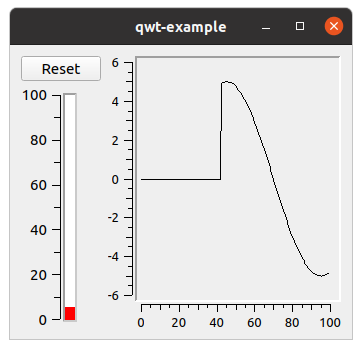
\includegraphics[width=0.5\textwidth]{qwtex}}
\end{center}
\caption{QT example layout
\label{qwtex}}
\end{figure}

There are different ways of declaring layout in QT. One is
using a markup language which then has matching classes
or creating it all with classes. We show how it works by
just using classes which organise the layout. There is
also a trend in general to use code to declare the layout
as done in SwiftUI, for example.

This is an example how widgets are organised into
nested vertical and horizontal layouts (see Fig.~\ref{qwtex}
for the result).
\begin{verbatim}
// create 3 widgets
button = new QPushButton;
thermo = new QwtThermo; 
plot = new QwtPlot;

// vertical layout
vLayout = new QVBoxLayout;
vLayout->addWidget(button);
vLayout->addWidget(thermo);

// horizontal layout
hLayout = new QHBoxLayout;
hLayout->addLayout(vLayout);
hLayout->addWidget(plot);

// main layout
setLayout(hLayout);
\end{verbatim}


\section{Callbacks in QT}
\subsection{Events from widgets}
In contrast to our low level callback mechanism using interfaces QT rather
directly calls methods in classes. The problem is that function pointers
cannot be directly used as a class has instance pointers to its local
data. So a method of a class needs to be combined with the instance
pointer. The QT method ``connect'' does exactly that:
\begin{verbatim}
connect(button,&QPushButton::clicked,
        this,&Window::reset);
\end{verbatim}
The QPushButton instance ``button'' has a method called ``clicked'' which is
called whenever the user clicks on the button. This is then forwarded to the
method ``reset'' in the application Widget.


\subsection{Plotting realtime data arriving via a callback}
The general idea is to store the realtime samples from a callback in a
buffer and trigger a screen refresh at a lower rate for example every
40~ms which then plots the contents of the buffer.

The callback ``addSample'' here is called in realtime whenever
a sample has arrived:
\begin{verbatim}
void Window::addSample( float v ) {
    // add the new input to the plot
    memmove( yData, yData+1, (plotDataSize-1) * sizeof(double) );
    yData[plotDataSize-1] = v;
}
\end{verbatim}
which stores the sample `v` in the shift buffer `yData`.

Then the screen refresh (which is slow) is done at
a lower and unreliable rate:
\begin{verbatim}
void Window::timerEvent( QTimerEvent * )
{
    curve->setSamples(xData, yData, plotDataSize);
    plot->replot();
    thermo->setValue( yData[0] );
    update();
}
\end{verbatim}

After ``update()'' has been called in the timer event the
paint event is executed by QT as soon as possible and re-paints
the canvas of the widget:
\begin{verbatim}
void ScopeWindow::paintEvent(QPaintEvent *) {
        QPainter paint( this );

        paint.drawLine( ... )
}
\end{verbatim}

Note that neither the timer nor the ``update()'' function
is called in a reliable way but whenever QT likes to do it.
So the QT timers cannot be used to sample data but should
only be used for screen refresh.



\chapter{Realtime webserver/client communication}

\section{Introduction}

Web server / client applications are at the heart of a huge number
of web applications ranging from shopping baskets to social
media applications.

Generally it's easy to create dynamic content
with many different solutions available (see PHP or nodejs) and well
documented. However, feeding realtime data from C++ to a web page or
realtime button presses back to C++ is a bit more difficult.

Important to recognise where \textsl{events} are generated: it's
always the client (web browser, mobile app) which triggers an event,
be it sending data over to the server or requesting data. It's
always initiated by the client.

\section{REST}
The interface between a web client (browser, phone app) is usually
implemented as a Representational State Transfer Architectural (REST)
style API by communicating via an URL on a web server. The most important requirements
for this API are very general and won't define the actual data format:
\begin{enumerate}
\item\textbf{Uniform interface} Any device connecting to the URL should
  get the same reply. No matter if a web page or mobile phone
  requests the temperature of a sensor the returned format must always be the same.
\item\textbf{Client-server decoupling} The only information
  the client needs to know is the URL of the server to request data or send data.
\item\textbf{Statelessness} Each request needs to include all the
  information necessary and must not depend on previous requests. For
  example a request to a buffer must not alter the
  buffer but just read from it so that another user reading the buffer
  shortly after receives the same data.
\end{enumerate}
See \url{https://www.ibm.com/cloud/learn/rest-apis} for the complete
list of REST design principles.

\section{Data formats}
\subsection{Server $\to$ client: JSON (application/json)}
The most popular dataformat is JSON which is basically a
map of key/value pairs which can also be nested:
\begin{verbatim}
{
    temperature: [20, 21, 20, 19, 17],
    steps: 100,
    comment: "all good!"
}
\end{verbatim}
Since JSON is sort of readable text a web server can simply
generate that text send it over via http or https. There
is no difference except that the MIME format is now `application/json`
instead of html.

\subsection{Client $\to$ server: POST (application/x-www-form-urlencoded)}
When a website sends data back to the server it needs to encode it in the
form of a single text-line where the key/value pairs are combined with \&-signs:
\begin{verbatim}
temperature=20&steps=100&comment=all+good%33
\end{verbatim}
The receiver then has the task to entangle this stream into a suitable dataformat,
for example a map. All server side scripting languages
such as \texttt{PHP} or \texttt{node.js} have powerful functions to
decode these strings. In C/C++ \texttt{libcurl}
can be used for decoding.


\section{Server}
On the Linux system a web server needs to be set up. There are
a variety of different options available but we are focusing here
on the ones which can be used for C++ communication (i.e. CGI).

\subsection{Web servers (http/https)}

\begin{itemize}
  \item NGINX: Easy to configure but very flexible web server
  \item Apache: Hard to configure but safe option
  \item lighttpd: Smaller web server with a small memory footprint
\end{itemize}
Note that it's possible to run different web servers at the
same time where they then act as proxies for a central web
server visible to the outside world. In particular nginx
makes it very easy to achieve this.

\begin{figure}[h]
\begin{center}
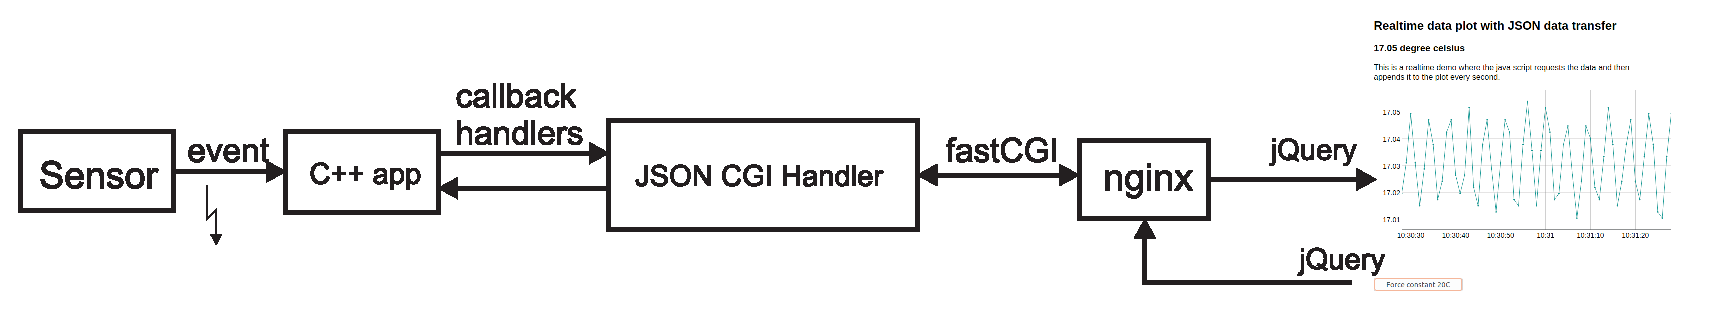
\includegraphics[width=\linewidth]{restdataflow}
\end{center}
\caption{FastCGI dataflow.\label{cgi}}
\end{figure}

\subsection{FastCGI}
FastCGI (see Fig~\ref{cgi}) is written in C++ and generates the entire
content of the http/https request. In particular here we generate
JSON packets serverside which can then be processed by client JavaScripts.
For realtime applications JSON transmission is perfect because the client-side
JavaScript can request JSON packages and directly turn them into variables.

A fast CGI program is a UNIX commandline program which communicates with the web server
(nginx, Apache, \ldots) via a UNIX socket which in turn is a pseudo file located
in a temporary directory for example `/tmp/sensorsocket`.

The web server then maps certain http/https requests to
his socket, for example, the configuration for nginx looks like this:
\begin{verbatim}
       location /sensor/ {
          include        fastcgi_params;
          fastcgi_pass   unix:/tmp/sensorsocket;
        }
\end{verbatim}
If the user does a request via the URL \texttt{www.mywebpage.com/sensor/} then
nginx contacts the fastcgi program via this socket. The fastcgi program
then needs to return the content. Internally this will be a C++ callback
inside of the fastcgi program.

The C++ fastcgi API \url{https://github.com/berndporr/json_fastcgi_web_api} 
is wrapper around the quite cryptic fastcgi C library and we are discussing
its callback handlers now.

\subsubsection{Server $\to$ client: JSON (application/json)}
The fastCGI callback expects a JSON string with the data
transmitted form the server to the client. There is helper
class JSONGenerator which generates the JSON data from various
C++ types:
\begin{verbatim}
class JSONcallback : public JSONCGIHandler::GETCallback {
public:
/**
* Gets the data and sends it to the webserver.
* The callback creates two JSON entries. One with the
* timestamp and one with the temperature from the sensor.
**/
virtual std::string getJSONString() {
    JSONCGIHandler::JSONGenerator jsonGenerator;
    jsonGenerator.add("epoch",(long)time(NULL));
    jsonGenerator.add("temperatures",temperatureArray);
    return jsonGenerator.getJSON();
    }
};
\end{verbatim} 

\subsection{Client $\to$ server: POST (application/x-www-form-urlencoded)}
Like in any GUI the client can press a button and create an event.
On the client side this is packaged as a JSON record with
jquery and then sent over to the server. The server then
receives the data as a callback:
\begin{verbatim}
virtual void postString(std::string postArg) {
		auto m = JSONCGIHandler::postDecoder(postArg);
		float temp = atof(m["volt"].c_str());
		std::cerr << m["hello"] << "\n";
		sensorfastcgi->forceValue(temp);
	}
\end{verbatim} 

\section{Client}
Generally on the client side (= web page) HTML with embedded
\textsl{JavaScript} is used to generate realtime output/input without
reloading the web page. JavaScript is \textsl{event driven} and has
callbacks so it's perfect for realtime applications. Use
\texttt{jQuery} to request and post JSON from/to the server.

For example here we request data from the server as a JSON
packet every second:

\begin{verbatim}
// callback when the JSON data has arrived
function getterCallback(result) {
  var temperatureArray = result.temperatures;
  // plot the array here
}

// timer callback (same idea as in QT to define a refresh rate)
function getTemperature() {
  // get the JSON data
  $.getJSON("/data/:80",getterCallback);
}

// document ready callback
function documentReady() {
  // request new data from the server every second
  window.intervalId = setInterval(getTemperature , 1000);
}

// called when the web page has been loaded
$(document).ready( documentReady );
\end{verbatim}


\chapter{Setters}

In Fig.~\ref{gettersetters} we have seen that data flows from
the sensors to the C++ classes via \textsl{callbacks}. The flow
back from inner C++ classes to motor or display outputs is via
\textsl{setters}. The same applies for setting configuration
parameters.

A setter is a simple method in a class, for example to set the
speed of a motor:
\begin{verbatim}
class Motor {
  /**
  * Set the Left Wheel Speed
  * @param speed between -1 and +1
  **/
  void setLeftWheelSpeed(float speed);
};
\end{verbatim}
Again as with callbacks it's important to abstract away from the
hardware, for example normalising the speed of the
motor and \textsl{hiding} away the complexity of the
PWM or GPIO ports in the class.

If a setter has more than one argument it's highly recommended
to use a \textsl{struct} to set the values.


\chapter{Data storage and memory management}

\section{Introduction}
Realtime processing should happen as quickly as possible. This means
that large memory allocations should happen at once. Small ones
are more effective as variables or \textsl{structs} which are passed as parameters
along a chain of callbacks or setters:
\begin{itemize}
\item Large memory allocation: Do all ``new'' commands at startup, ``delete'' at shutdown.
\item Small memory segments: variables or structs.
\end{itemise}





\end{document}
